
\chapter{Analysis}\label{chp:analysis}

\section{Impact of Jittered Masses on Viscosity and Structure}

A particularly interesting observation that ties the topic of lattices, random jitter and uniform densities together is the fact that for a uniform initial density combined with a jitter, the mass of the particles is necessarily non-uniform and varies pseudo-randomly. This actually appears to lead to defects in the formation of the crystalline structures that otherwise naturally form, as seen in \autoref{fig:natural-hexagons}, resulting instead in a more amorphous structure. This could have desirable effects, such as increasing isotropy or perhaps reducing undesired viscosity. Intuitively, a particle in a crystalline structure may be expected to require more energy to be moved along an arbitrary direction, than if it had settled into a less rigid structure.

To test this hypothesis, a scene very similar to the Taylor-Green vortex was used, where fluid is initialized at rest density using some lattice as described above, but given a varying degree of pseudo-random jitter in the initial positions. The fluid is contained in a box with no gravity, where all viscosities are in this case set to zero in order to measure only the undesired loss in kinetic energy inherent to the simulation method. The particles are initialized with a velocity that varies according to a sine and cosine function of positions $\vek{x}_i$ such that four opposing vortices form in each of the four quadrants of a $[0;2\pi]^2$ domain, using in this case\autocite*{taylor-green-arxiv}:

\begin{equation}
  \vek{v}(t=0)_i = 2\begin{pmatrix}
    \sin(x_i) \cos(y_i) \\
    -\cos(x_i) \sin(y_i)
  \end{pmatrix}
\end{equation}
where $\vek{x}_i = (x_i, y_i)^T$. The setting is visualized in \autoref{fig:taylor-green-vortex}, where colour-coded particles are advected.

\begin{figure}
  \centering
  \begin{subfigure}[t]{0.4\textwidth}
    \includegraphics[width=\textwidth]{images/density/taylorgreen_t0.jpg}
    \caption{$t=0s$}
  \end{subfigure}
  \begin{subfigure}[t]{0.4\textwidth}
    \includegraphics[width=\textwidth]{images/density/taylorgreen_t4_70.jpg}
    \caption{$t=4.7s$}
  \end{subfigure}
  \caption{$95 500$ colour coded particles are advected by a Taylor-Green vortex on a $[0;2\pi]$ domain, with four vertices each spinning in directions opposite to their respectively adjacent vortices.}
  \label{fig:taylor-green-vortex}
\end{figure}

The rate at which the velocity of the Taylor-Green vortex on a periodic domain decays in relation to the viscosity of a fluid is analytically known to be\autocite*{taylor-green-arxiv} in $\mathcal{O}\br{e^{-\nu t}}$. Despite the exact analytic solution not holding in this instance since periodic boundaries are not applied, the scenario still allows the comparison of decay of the average kinetic energy in the system for different initial samplings of the fluid, where a slower decay is more desirable in reaching lower effective viscosities. A $\frac{1}{N}E_{kin}(t)$ curve can be plotted for different initial sampling lattices and amounts of jitter in conjunction with uniform initial density as described in \autoref*{sec:equilibrate-density}, which is shown in \autoref{fig:taylor-green-result}


\begin{figure}
  \centering
  \begin{tikzpicture}
    \begin{axis}[
      xlabel={Time $t$},
      ylabel={Average Kinetic Energy $\frac{1}{N}E_{kin}(t)$},
      legend pos=south west,
      legend style={font=\small, cells={anchor=west}}, % Make legend smaller and more compact
      grid=none,
      no markers,
      every axis plot/.append style={ultra thin},
      axis line style={-},
      tick align=outside,
      tick style={thin, black},
      clip=false,
      enlarge x limits=0, % remove padding
      enlarge y limits=0, % remove padding
      width=\textwidth
      ]

      \addplot [color=Spectral0] table [x=hex_0jitterx, y=hex_0jittery, col sep=comma] {taylor_avg_ekin_over_t.csv};
      \addlegendentry{Hexagonal Lattice, $\sigma=0h$}

      \addplot [color=Spectral1] table [x=hex_1jitterx, y=hex_1jittery, col sep=comma] {taylor_avg_ekin_over_t.csv};
      \addlegendentry{Hexagonal Lattice, $\sigma=0.01h$}

      \addplot [color=Spectral2] table [x=hex_5jitterx, y=hex_5jittery, col sep=comma] {taylor_avg_ekin_over_t.csv};
      \addlegendentry{Hexagonal Lattice, $\sigma=0.05h$}

      \addplot [color=Spectral3] table [x=reg_1jitterx, y=reg_1jittery, col sep=comma] {taylor_avg_ekin_over_t.csv};
      \addlegendentry{Square Lattice, $\sigma=0.01h$}

      \addplot [color=Spectral4] table [x=reg_5jitterx, y=reg_5jittery, col sep=comma] {taylor_avg_ekin_over_t.csv};
      \addlegendentry{Square Lattice, $\sigma=0.05h$}

    \end{axis}
  \end{tikzpicture}

  \caption*{\begin{tiny}$\nu=\nu_2=0, k=1000, h=0.033, \lambda=0.1, N=90500K, \vec{x}\in[0;2\pi]^2, v_{x_0} = 2\sin (x)\cos (y), v_{y,0} = -2\cos (x)\sin (y), \rho_0 = 1$ \texttt{SplitSPH}\end{tiny}}
  \caption{Time evolution of $E_{kin}$ in Taylor-Green vortex for varying amounts of initial jitter and initial sampling lattices. As the initial Jitter approaches a standard deviation of 5\% of the particle spacing $h$, there is a continuous decrease in undesired viscosity. The hexagonal lattice being the most stable in many a sense is detrimental in this case, where to achieve low viscosities, a small jitter and an initial square-lattice sampling appear more effective.}
  \label{fig:taylor-green-result}
\end{figure}



\begin{samepage}


  \autoref{fig:taylor-green-result} suggests that viscosity does in fact decrease as the mass varies more intensely, at least up to a reasonable amount of initial jitter.
  In order to empirically examine whether this is actually due to fewer rigid, crystalline structures forming, a metric for the degree of crystallinity or amorphousness of a material, or in other words a structural order parameter, is required. For this, a metric from the study of two-dimensional melting in condensed matter physics may be borrowed: the Nelson-Halperin 2D bond orientational order parameter\autocite*{bond-orientational-parameter-pis-6} $\Psi_6$. It is defined as\autocite{nature-psi-6-bond-orientational}:
  \begin{equation}
    \Psi_6^k = \frac{1}{n_k} \sum_{l\in\mathcal{N}(k)}e^{6i\Theta_{k,l}}
  \end{equation}
  where the sum is over the $n_k$ nearest neighbours $k\neq l$ to the particle of index $k$ determined through a Delaunay triangulation, $\Theta_{k,l}$ is the angle between particles $k,l$ measured from an arbitrary, fixed axis and the usual particle index $i$ was avoided to not cause confusion with the imaginary unit in the exponent \autocite*{nature-psi-6-bond-orientational}. Generally, the $\Psi_x$ metric shows how close to perfect $x$-atic symmetry the local environment is, which is why the hexatic $\Psi_6$ metric was chosen for this two-dimensional case where the hexagon is the unique closest packing and six nearest neighbours are indeed the most frequent result of a Delaunay triangulation of the particle positions for all simulation runs. The value $0 \leq \abs{\Psi_6} \leq 1$ is maximized for a hexagonal grid and decreases as the material becomes less ordered\autocite*{nature-psi-6-bond-orientational}, where magnitude expresses regularity or how 'well-packed' the arrangement is\autocite*{nicer-psi-6-bond-orientational}, while the complex number itself also encodes a phase or orientation of the structure.

  If there was a relation between jittered masses, lower viscosity and preventing crystal structures, one would expect the average magnitude of the bond orientation parameter $\Psi_6^{avg} = \frac{1}{N}\sum_i \abs{\Psi_6^i}$ to decrease as the jitter increases and the material becomes more disorderly. To test this, $\Psi_6^{avg}$ was measured at $t=30$ for all the configurations in \autoref{fig:taylor-green-result}, as long as possible after the initialization:

  \begin{center}
    \begin{tabular}{|c | c | c || c|}
      \hline
      Lattice   & Time & Jitter $\sigma$ & $\Psi_6^{avg}$ \\
      \hline\hline
      Hexagonal & t=0  & 0               & 0.973          \\\hline
      Hexagonal & t=30 & 0               & 0.522          \\\hline
      Hexagonal & t=30 & 0.01h           & 0.511          \\\hline
      Hexagonal & t=30 & 0.05h           & 0.459          \\\hline
      Square    & t=30 & 0.01h           & 0.478          \\\hline
      Square    & t=30 & 0.05h           & 0.444          \\\hline
    \end{tabular}

  \end{center}
\end{samepage}

As can be seen, irrespective of which lattice is used to sample the fluid, there are more defects, less order and therefore lower values of $\Psi_6^{avg}$ as the jitter increases, even long after the initial conditions should have no more bearing on the behaviour of the fluid. This further suggests that the combination of jitter and solving for uniform density could indeed make the discretization more isotropic and help decrease unwelcome viscosity. On the other hand, especially for small kernel support radii, the SPH approximation quality might suffer from excessive particle disorder.

Just to further drive home the point that order decreases as particle masses vary, the Voronoi tessellations of the particle positions from the same simulation runs can be analysed instead of $\Psi_6$. Then, particles the Vornoi cells of which form a polygon with six vertices, more than six or less than six vertices can be coloured respectively and plotted, as seen in \autoref{fig:jitter-vornoi-tesselation}. This again suggests that jittered masses lead to more defects in otherwise locally ordered structures.

\begin{figure}
  \begin{subfigure}[t]{0.49\textwidth}
    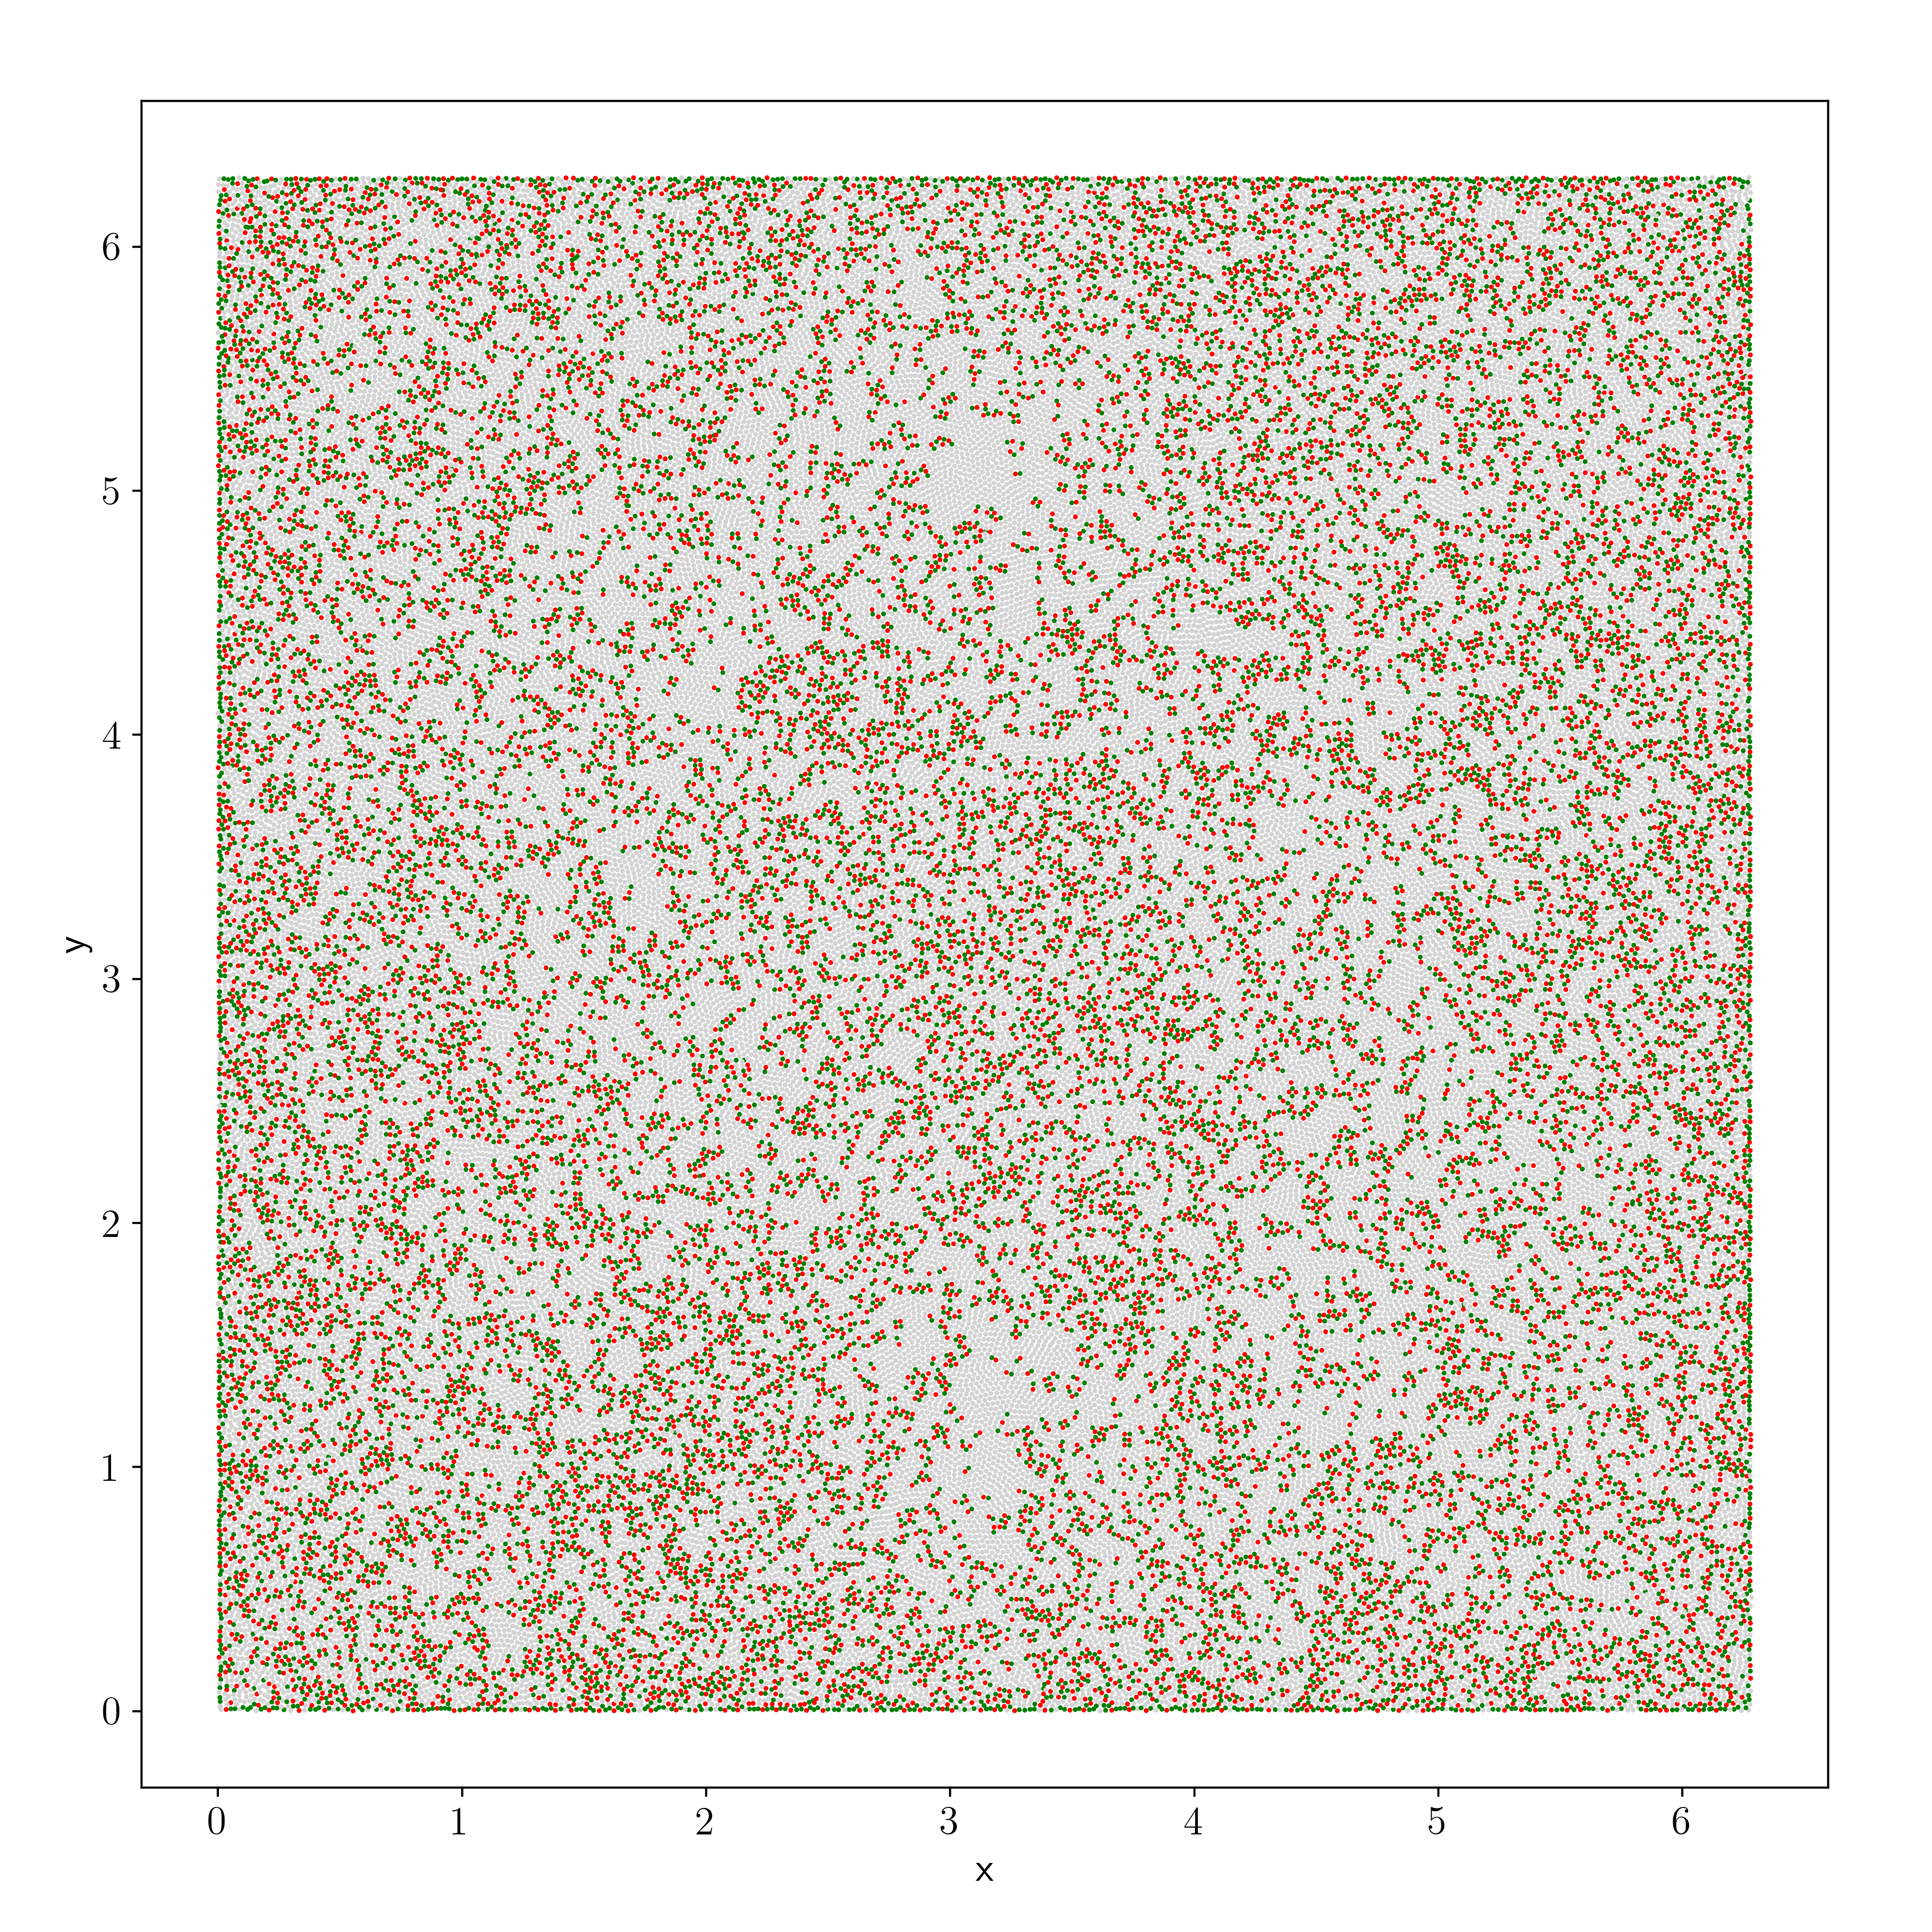
\includegraphics[width=\textwidth]{images/density/hex_0jitter_vornoi.png}
    \caption{$\sigma=0$}
  \end{subfigure}
  \begin{subfigure}[t]{0.49\textwidth}
    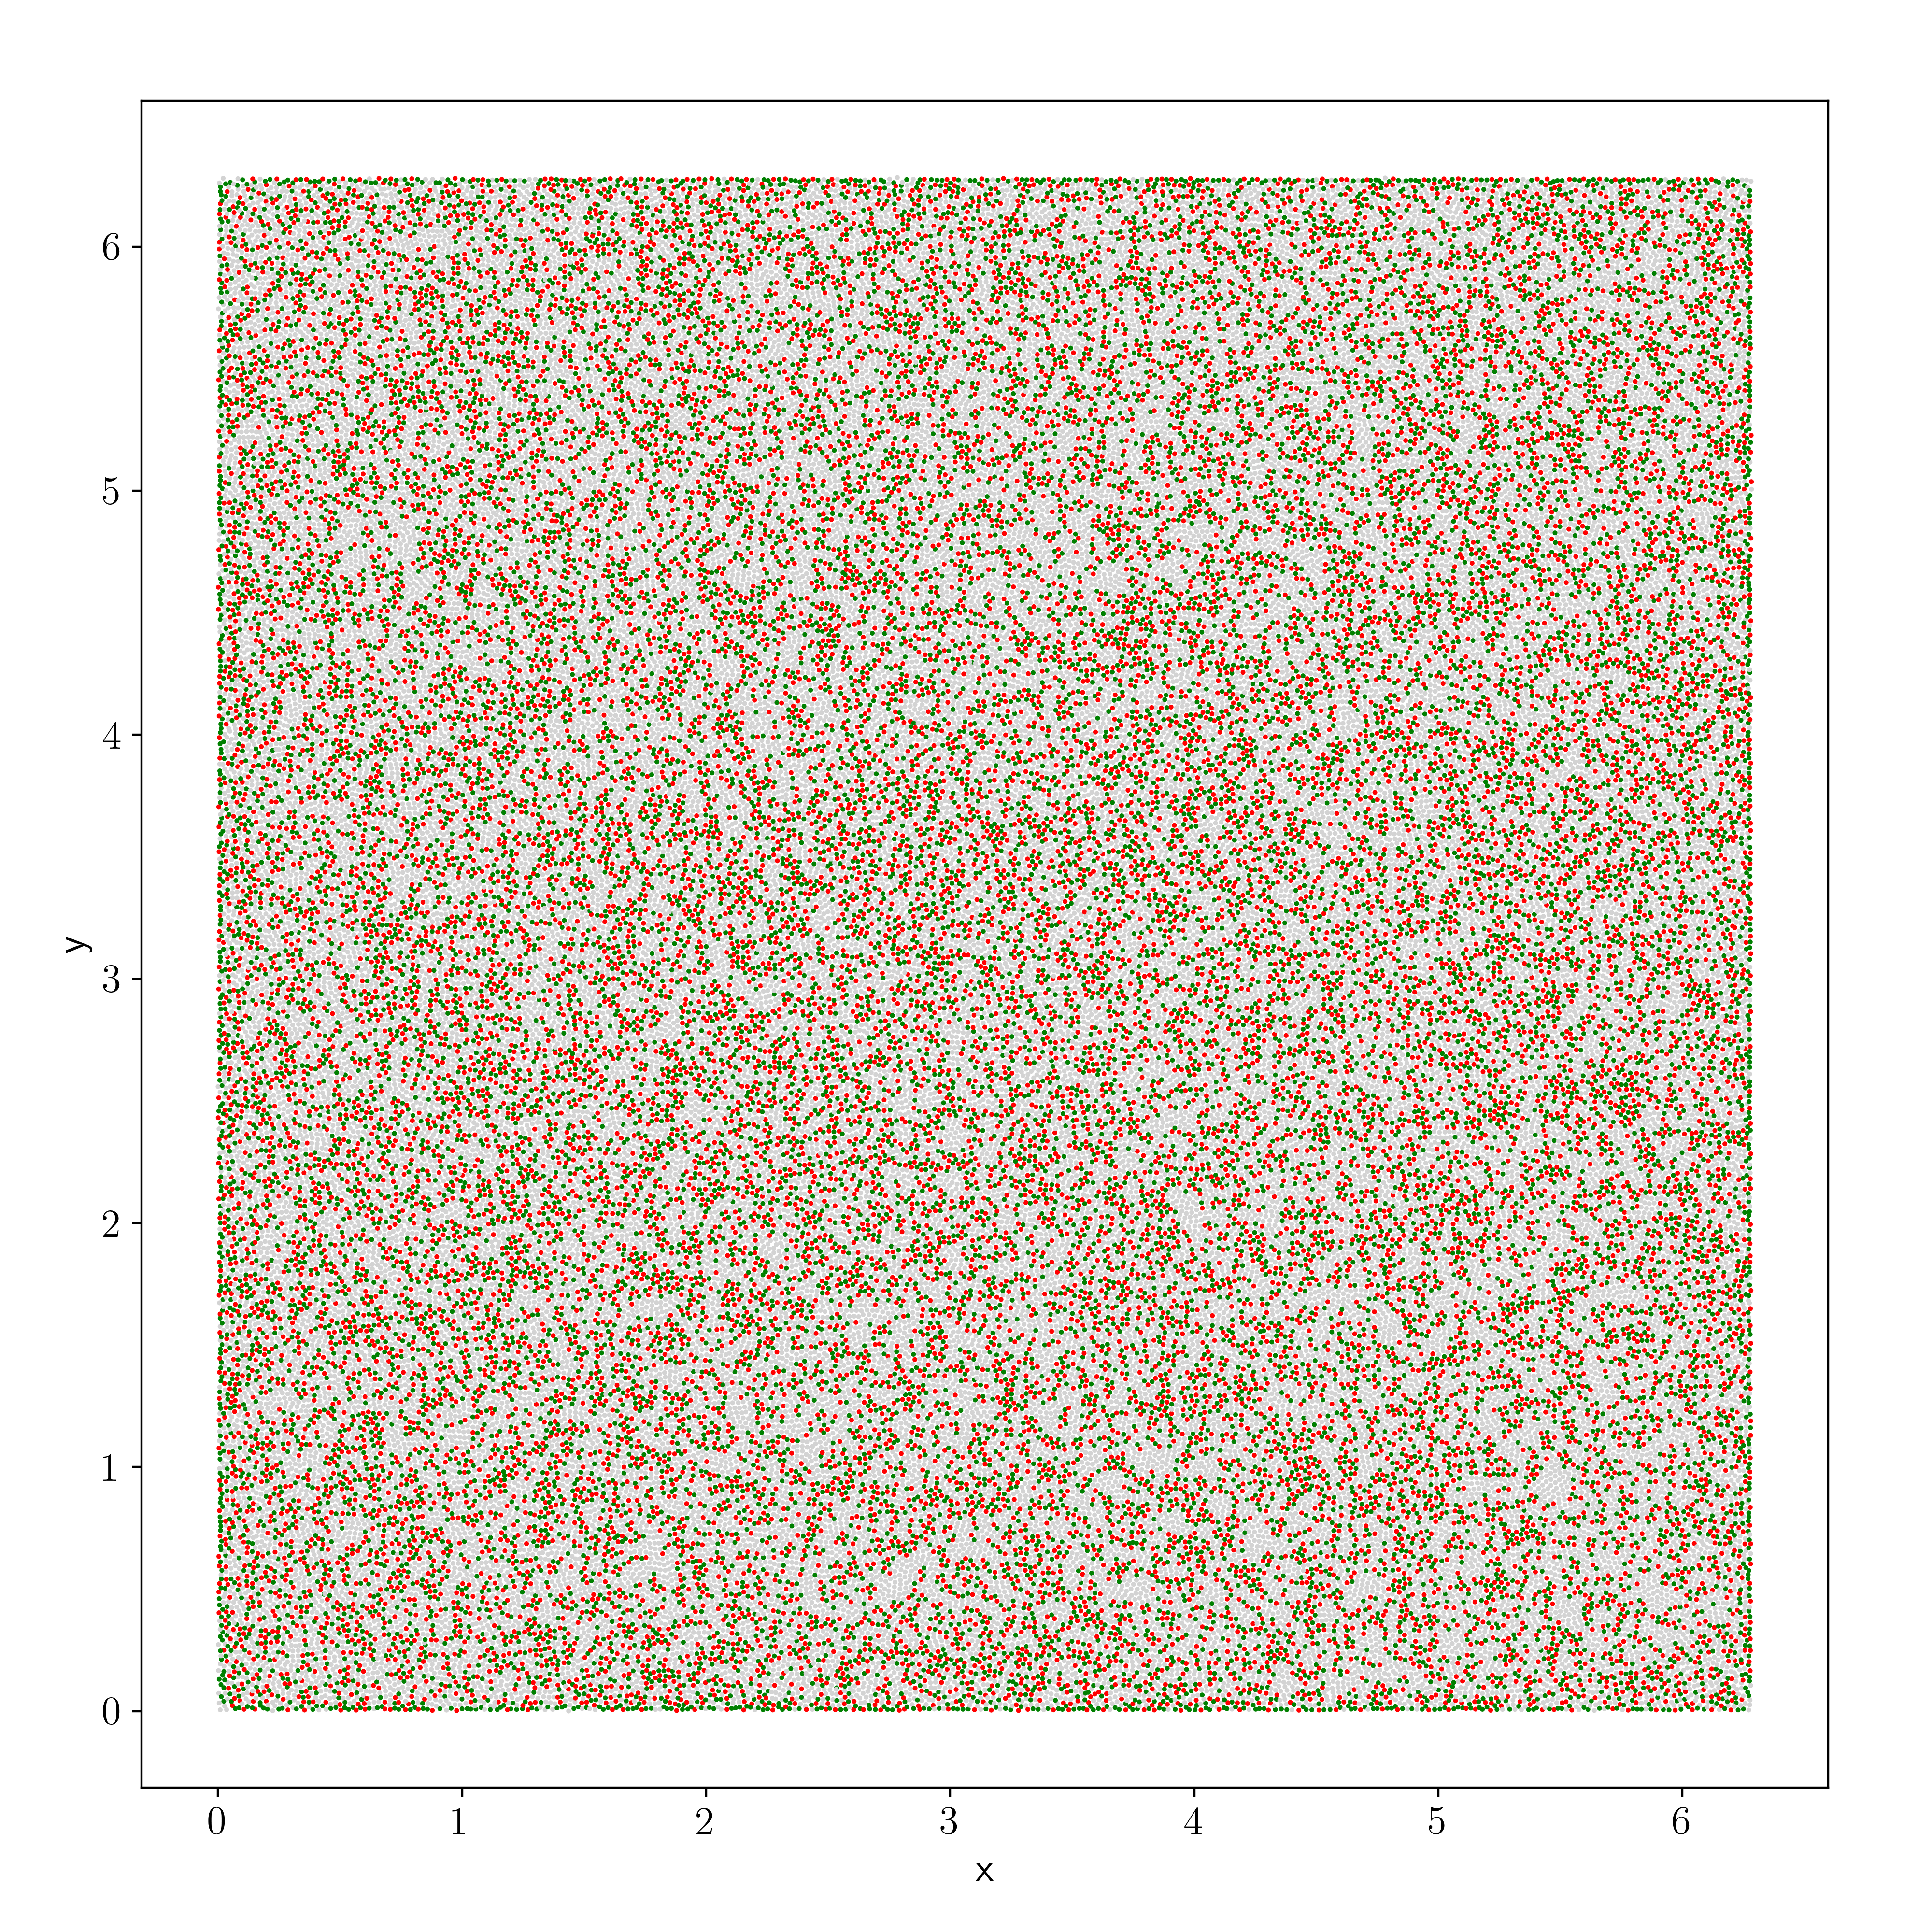
\includegraphics[width=\textwidth]{images/density/hex_5jitter_vornoi.png}
    \caption{$\sigma=0.05h$}
  \end{subfigure}
  \caption{The result of the Vornoi tessellation of the simulations of the Taylor-Green vortex are shown for a hexagonal initial sampling at $t=30$ with the specified jitter (all parameters are the same as in \autoref{fig:taylor-green-result}). Each particle that has a Voronoi cell with more than six vertices is coloured red, ones with fewer neighbours are coloured green. While for  $\sigma=0$, there are 61759 particles that have hexagonal Voronoi cells, for $\sigma=0.05h$ jitter there are only 52845 such particles, as can be seen observed in the increased amount of coloured dots in the right figure. This further suggests that pseudo-randomly varying particle masses create a less ordered and possibly more isotropic structure down the line.}
  \label{fig:jitter-vornoi-tesselation}
\end{figure}

In sources on melting of condensed matter in two dimensions, the hexatic phase is frequently examined, creating a continuous middle ground between the solid and liquid phases and bearing a surface-level resemblance to the structures seen in \autoref{fig:natural-hexagons} - it might be interesting to draw from knowledge about these physical processes in order to combat undesired viscosity in SPH fluid simulation and reach higher Reynolds numbers, analysing for example the time evolution of translational and orientational order throughout a simulation and how masses and kernel support radii that vary per particle or resampling of fields can influence these phenomena - however those analyses are not conducted in this report.


\newpage
\section{Oscillation Frequency and Error as a Function of Stiffness}\label{sec:oscillations}
By choosing a density invariance term in the formulation of the fluid solvers instead of the velocity divergence, the fluid can be expected to oscillate about its rest density for the non-iterative solvers \texttt{SplitSPH} and \texttt{EOSSPH} instead of exhibiting volume drift.


The iterative solver behaves somewhat similarly, but does not oscillate about the rest density in a sinusoidal fashion since incompressibility is more strongly enforced with a density error threshold that the average density does not significantly exceed, resulting in peaks of the oscillations in density being cut off. To make the \texttt{IterSPH} solver more comparable, a fixed amount of iterations can be used, $l_{iter}=l_{min}=l_{max}=3$ in this case, which makes the oscillation regular but disables any error thresholds or guarantees.

One can analyse the behaviour of this oscillating error using a simple column of water in a tall, rectangular container, since it is known that this configuration would ideally result in a perfectly still fluid that does not oscillate. The width of the container has little bearing on the magnitude of the error, which is why a narrow and tall configuration is preferred in order to analyse the same effect using fewer particles and therefore less computation time. Both the amplitude and the frequency of this oscillation can be found to depend on the stiffness parameter $k$ that governs incompressibility in the equation of state. In this section, the influence of $k$ on the magnitude of the error and the frequency of the oscillation are analysed. The setting and the oscillation are shown in \autoref{fig:oscillating-column}

\begin{figure}[h]
  \centering
  \begin{subfigure}[t]{0.09\textwidth}
    \includegraphics[width=\textwidth]{images/oscillate/000.jpg}
    \caption{\small{$t=0.0s$}}
  \end{subfigure}%
  \begin{subfigure}[t]{0.09\textwidth}
    \includegraphics[width=\textwidth]{images/oscillate/020.jpg}
    \caption{\small{$t=0.2s$}}
  \end{subfigure}%
  \begin{subfigure}[t]{0.09\textwidth}
    \includegraphics[width=\textwidth]{images/oscillate/030.jpg}
    \caption{\small{$t=0.3s$}}
  \end{subfigure}%
  \begin{subfigure}[t]{0.09\textwidth}
    \includegraphics[width=\textwidth]{images/oscillate/040.jpg}
    \caption{\small{$t=0.4s$}}
  \end{subfigure}%
  \begin{subfigure}[t]{0.09\textwidth}
    \includegraphics[width=\textwidth]{images/oscillate/050.jpg}
    \caption{\small{$t=0.5s$}}
  \end{subfigure}%
  \begin{subfigure}[t]{0.09\textwidth}
    \includegraphics[width=\textwidth]{images/oscillate/060.jpg}
    \caption{\small{$t=0.6s$}}
  \end{subfigure}%
  \begin{subfigure}[t]{0.09\textwidth}
    \includegraphics[width=\textwidth]{images/oscillate/070.jpg}
    \caption{\small{$t=0.7s$}}
  \end{subfigure}%
  \begin{subfigure}[t]{0.09\textwidth}
    \includegraphics[width=\textwidth]{images/oscillate/080.jpg}
    \caption{\small{$t=0.8s$}}
  \end{subfigure}%
  \begin{subfigure}[t]{0.09\textwidth}
    \includegraphics[width=\textwidth]{images/oscillate/090.jpg}
    \caption{\small{$t=0.9s$}}
  \end{subfigure}%
  \begin{subfigure}[t]{0.09\textwidth}
    \includegraphics[width=\textwidth]{images/oscillate/100.jpg}
    \caption{\small{$t=1.0s$}}
  \end{subfigure}
  \caption*{\begin{tiny}$k=100, \nu=0.01, \nu_2=0, h=0.02, \lambda=0.1, N=1572, \rho_0 = 1, \Delta t = 0.0002s$ \texttt{SplitSPH}\end{tiny}}
  \caption{A half-filled, tall, rectangular tube is shown with the density of the fluid being colour-coded. For the very small stiffness parameter $k=100$ shown here, major compressions occur and a clearly visible, slow oscillation sets in.}
  \label{fig:oscillating-column}
\end{figure}

The effect can be thought of as an oscillation due to the fact that particles at the top of the column are still in free fall when the bottom particles first experience contact forces - the stiffer the fluid, the faster the shock within it propagates and the quicker the particles at the top of the column are accelerated back up, where gravity takes over and the cycle continues, albeit with smaller and smaller amplitude.

In order to conduct the analysis, the measured density according to \autoref{eq:density-sph} can be averaged across all particles to obtain $\rho_{avg}(t) = \frac{1}{N}\sum_i \rho_i(t)$, and the rest density subtracted to obtain the average density error $\Delta \rho(t) = \rho_{avg}(t)-\rho_0$, which oscillates about zero. This is done for a simulation running with a specified, fixed time step $\Delta t$; the CFL-condition is not used in favour of obtaining a regular sampling of the $\Delta \rho(t)$-Curve which can be more easily subjected to a discrete Fourier transform to analyse the frequency of the oscillation. In the following, a time step size of $\Delta t = 0.0002s$ is used, which is a conservative estimate of the $\Delta t$ required by the CFL condition. This means that $\Delta \rho(t)$ is sampled at $5000Hz$ and the frequency:
\begin{equation}
  f_{peak}=\argmax_{f}\mathcal{F}\br{\Delta \rho(t)} = \argmax_{f}\Delta\rho'(f)
\end{equation}
with maximum contribution to the spectrum of the oscillation is plotted against $k$, neglecting the zero-frequency $f_0$ which is plotted in a separate graph and expresses the magnitude of the total error. This is done for $2s\leq t\leq 12s$, where the first two seconds of simulated time are discarded in order to minimize the impact of the initial configuration.

\begin{figure}[hbt]
  \begin{tikzpicture}
    \begin{axis}[
        xlabel={Stiffness $k$},
        ylabel={Peak oscillation frequency $f_{peak} (Hz)$},
        legend pos=north west,
        legend style={font=\small, cells={anchor=west}}, % Make legend smaller and more compact
        grid=none,
        no markers,
        every axis plot/.append style={ultra thin},
        axis line style={-},
        tick align=outside,
        tick style={thin, black},
        clip=false,
        enlarge x limits=0, % remove padding
        enlarge y limits=0, % remove padding
        width=\textwidth,
        height=0.7\textwidth,
        % xmode=log,
        % ymode=log,
      ]

      \addplot [color=Spectral0, thick] table [x=k, y=EOSSPHhighvis, col sep=comma] {k_to_freq.csv};
      \addlegendentry{\texttt{EOSSPH}, $\nu=10^{-2}$}
      \addplot [color=Spectral2, dashed] table [x=k, y=EOSSPHlowvis, col sep=comma] {k_to_freq.csv};
      \addlegendentry{\texttt{EOSSPH}, $\nu=10^{-3}$}

      \addplot [color=Spectral3, thick] table [x=k, y=SplitSPHhighvis, col sep=comma] {k_to_freq.csv};
      \addlegendentry{\texttt{SplitSPH}, $\nu=10^{-2}$}
      \addplot [color=Spectral7, dashed] table [x=k, y=SplitSPHlowvis, col sep=comma] {k_to_freq.csv};
      \addlegendentry{\texttt{SplitSPH}, $\nu=10^{-3}$}

      \addplot [color=Spectral8, thick] table [x=k, y=IterSPHhighvis, col sep=comma] {k_to_freq.csv};
      \addlegendentry{\texttt{IterSPH}, $\nu=10^{-2}$}
      \addplot [color=Spectral10, dashed] table [x=k, y=IterSPHlowvis, col sep=comma] {k_to_freq.csv};
      \addlegendentry{\texttt{IterSPH}, $\nu=10^{-3}$}
      \addplot [color=red] table [x=k, y=prediction, col sep=comma] {k_to_freq.csv};
      \addlegendentry{Prediction}

    \end{axis}
  \end{tikzpicture}
  \caption*{\begin{tiny}$\nu_2=0.001, h=0.02, \Delta t = 0.0002s, N=1572, \rho_0 = 1, \gamma_1=1, \gamma_2=0.5$, Hexagonal sampling with $\sigma=0.015h$\end{tiny}}
  \caption{The frequency $f_{peak}$ with maximum contribution to the oscillation of the function $\Delta\rho (t)$ is plotted against the stiffness parameter $k$ that governs incompressibility. The frequency of oscillation continuously increases as $k$ increases. The four lowest curves, corresponding to all \texttt{EOSSPH} and \texttt{SplitSPH} simulations, all overlap.}
  \label{fig:freq-peak-k}
\end{figure}

The results of the frequency analysis are shown in \autoref{fig:freq-peak-k}.
This graph shows that as the stiffness $k$ increases, so does the frequency of the oscillation. The graph closely resembles a square root function, which might be explained by the stiffness being linked to the \emphasis{numerical speed of sound} $c$, which governs the frequency of the oscillations\autocite*{speed-of-sound-k}, through the Newton-Laplace equation that states\autocite*{speed-of-sound}:
\begin{equation}\label{eq:newton-laplace}
  c = \sqrt{\frac{\Delta p}{\Delta\rho}}
\end{equation}
meaning that for the equation of state in \autoref{eq:state-equation} for which $\Delta p \propto k\Delta\rho$ and if the oscillation frequency is indeed proportional to the numerical speed of sound ($f_{peak} \propto c$), then:
\begin{equation}
  f_{peak}
  \propto c
  = \sqrt{\frac{\Delta p}{\Delta\rho}}
  \propto \sqrt{\frac{k \Delta\rho}{\Delta\rho}}
  = \sqrt{k}
\end{equation}
and therefore $f_{peak} \propto \sqrt{k}$, which would explain the shape of the curve.

The graph also clearly shows that the oscillation is \textit{not affected} by viscosity, with simulations that differ in $\nu$ by an order of magnitude exactly overlapping, and that operator splitting \textit{also does not affect} the result at all. This further evidences that the oscillation frequency depends on the numerical speed of sound and not any of the other factors mentioned. The only solver with a differing curve is the iterative solver: for this solver, one would expect the numerical speed of sound to be higher, since there are multiple iterations per time step that may propagate information, or accelerations, from neighbouring particle to neighbouring particle - this makes intuitive sense, since the iterative solver achieves a higher effective incompressibility, which has been shown to be linked to the numerical speed of sound in \autoref{eq:newton-laplace}.


One could speculate that within some low bound of $l_{iter}$, where repeated neighbourhood calculations are not necessary, the number of iterations could have a nearly linear relationship with the stiffness $k$, the square root of which was assumed above to be proportional to the frequency of oscillation - if this were true, one would expect the iterative solver with $l_{iter}=3$ to have a higher frequency of oscillation by a factor of $\sqrt{l_{iter}}=\sqrt{3}$.
To test this hypothesis, the average of the four curves using a single-iteration solver in \autoref{fig:freq-peak-k} was taken, a square root function fitted to this average using the Levenberg-Marquardt algorithm for least squares regression\footnote{Implemented in SciPy Optimize: Curve Fit \url{https://docs.scipy.org/doc/scipy/reference/generated/scipy.optimize.curve_fit.html}} and then multiplied by $\sqrt{3}$ to yield the red line shown in \autoref{fig:freq-peak-k} as the \textit{Prediction}. This curve describes what would be expected to happen if the hypotheses made in this section were true, meaning:
\begin{enumerate}
  \item $f_{peak}\propto\sqrt{k}$
  \item  $k\propto l_{iter}$
\end{enumerate}
and matches the experimental values for the $l=3$ solver remarkably well, suggesting that stiffness may indeed be almost linear in the number of iterations for such solvers, at least up to some small, fixed number of iterations.

\horizontalspacer


The total density error across time can be expressed by the zero-frequency $f_0$ of the discrete Fourier transform of $\Delta\rho (t)$ as shown in \autoref{fig:error-to-k}, where:
\begin{equation}
  f_0 = \int_{2s}^{10s} \Delta\rho (t) \,dt
\end{equation}
Note that $\Delta\rho (t)$ should oscillate about zero, so the integral should be zero if the solver perfectly enforces incompressibility, greater than zero if some compression occurs and negative if somehow the measured average density across particles and time is below rest density.

Here, the data shows that a greater stiffness coefficient $k$ results in less density error, which makes sense since compressions for higher $k$ result in greater pressure forces that correct the compression.

The graph also shows how increasing the stiffness $k$ yields diminishing returns, further motivating the use of iterative solvers as a way to improve simulation quality, since simply increasing the stiffness used in a single iteration per time step might become unfeasible. The iterative solver with three iterations achieves a much smaller value of $f_0$ across all coefficients $k$.

In this instance, the single-iteration solvers with and without operator splitting again show the same behaviour, with viscosity once more playing no role in the oscillation for the measured range of parameters. Operator splitting, while perhaps effective in reducing some kinds of errors and improving robustness and stability, does not have an impact on the type of error under consideration in this scenario.


At some point, when increasing $k$, instability might occur if the time step size $\Delta t$ is not simultaneously decreased, making the simulation more computationally expensive - this is analysed in the following section.


\begin{figure}[hbt]
  \begin{tikzpicture}
    \begin{axis}[
        xlabel={Stiffness $k$},
        ylabel={Zero Frequency $f_{0}$},
        legend pos=north east,
        legend style={font=\small, cells={anchor=west}}, % Make legend smaller and more compact
        grid=none,
        no markers,
        every axis plot/.append style={ultra thin},
        axis line style={-},
        tick align=outside,
        tick style={thin, black},
        clip=false,
        enlarge x limits=0, % remove padding
        enlarge y limits=0, % remove padding
        width=\textwidth,
        height=0.7\textwidth,
        % xmode=log,
        % ymode=log,
      ]

      \addplot [color=Spectral0, thick] table [x=k, y=EOSSPHhighvis, col sep=comma] {k_to_error.csv};
      \addlegendentry{\texttt{EOSSPH}, $\nu=10^{-2}$}
      \addplot [color=Spectral2, dashed] table [x=k, y=EOSSPHlowvis, col sep=comma] {k_to_error.csv};
      \addlegendentry{\texttt{EOSSPH}, $\nu=10^{-3}$}

      \addplot [color=Spectral3, thick] table [x=k, y=SplitSPHhighvis, col sep=comma] {k_to_error.csv};
      \addlegendentry{\texttt{SplitSPH}, $\nu=10^{-2}$}
      \addplot [color=Spectral7, dashed] table [x=k, y=SplitSPHlowvis, col sep=comma] {k_to_error.csv};
      \addlegendentry{\texttt{SplitSPH}, $\nu=10^{-3}$}

      \addplot [color=Spectral8, thick] table [x=k, y=IterSPHhighvis, col sep=comma] {k_to_error.csv};
      \addlegendentry{\texttt{IterSPH}, $\nu=10^{-2}$}
      \addplot [color=Spectral10, dashed] table [x=k, y=IterSPHlowvis, col sep=comma] {k_to_error.csv};
      \addlegendentry{\texttt{IterSPH}, $\nu=10^{-3}$}

    \end{axis}
  \end{tikzpicture}
  \caption*{\begin{tiny}$\nu_2=0.001, h=0.02, \Delta t = 0.0002s, N=1572, \rho_0 = 1, \gamma_1=1, \gamma_2=0.5$, Hexagonal sampling with $\sigma=0.015h$\end{tiny}}
  \caption{The zero frequency $f_0$ or integral of the function $\Delta\rho (t)$ is plotted against the stiffness parameter $k$ that governs incompressibility. As the stiffness increases, the total error sharply decreases. The viscosity and whether operator splitting is applied has no impact on the single-iteration solvers \texttt{EOSSPH} and \texttt{SplitSPH}, the curves of which all overlap. The \texttt{IterSPH} solver with three iterations achieves a lower total error across all $k$.}
  \label{fig:error-to-k}
\end{figure}

\newpage

\section{Stability as a Function of Viscosity, Stiffness and Time Step Size}
The setting described in \autoref{sec:oscillations}, where a column of water at rest is simulated, can also be used to analyse the stability of the simulation. Once again, the fact that the water ought to be at rest and therefore the analytic solution is trivially known can be used to measure an error $\epsilon$ relative to that solution for each of the solvers presented in \autoref{chp:solvers}. It has already been discussed that higher stiffness $k$ can lead to better simulation accuracy, but it has not yet been shown that a choice of $k$ that is too large for a given time step size $\lambda$ can lead to unstable behaviour with erratically moving particles and unphysical behaviour. Ideally, the average kinetic energy of the fluid particles $E_{kin}(t) = \frac{1}{N}\sum_i m_i \dist{\vek{v}_i(t)}^2$ is at zero, or very close to it, for the resting water column shown in \autoref{fig:oscillating-column}. Instabilities can be detected by the kinetic energy being considerably higher than expected and repeatedly spiking, which is measured in the following using the logarithm of the average \emphasis{action} of the particles, assuming a potential energy of zero:
\begin{equation}\label{eq:action-log-error}
  \epsilon = \log_{10}\br{\int_{10s}^{20s} E_{kin}(t) \,dt}
\end{equation}
where the first 10 seconds are discarded to make sure that any movement due to unfortunate initial conditions and the oscillations measured in \autoref{sec:oscillations} have subsided, the state of the particles is somewhat equilibrated, and instabilities are responsible for any remaining, significant amounts of kinetic energy. The time integration in \autoref{eq:action-log-error} is implemented using the trapezoidal rule and the logarithm is taken to account for an unstable simulation potentially having multiple orders of magnitude more kinetic energy than a stable simulation in this scenario. The results are shown in \autoref{fig:stability-k-lambda}.


\begin{figure}
  \centering
  \begin{subfigure}[t]{\textwidth}
    \centering
    \begin{tikzpicture}
      \begin{groupplot}[
          group style={
              group size=2 by 3,
              vertical sep=2cm,
              horizontal sep=2cm,
            },
          colormap name=Spectral_r,
          % colormap/viridis, 
          point meta min=-1.9,
          point meta max=2.1,
          view={0}{90},
          xlabel={$k$},
          ylabel={$\lambda$},
          zlabel={$\epsilon$},
          width=0.45\textwidth,
          height=0.45\textwidth,
        ]
        \nextgroupplot[
          title={\texttt{EOSSPH}}
        ]

        \addplot3 [
          contour filled,
        ] table {500.0 0.1 -1.775406581727304
500.0 0.325 -1.774586966838677
500.0 0.55 -1.774586966838677
500.0 0.775 -1.774586966838677
500.0 1.0 -1.774586966838677

750.0 0.1 -1.0878262651867756
750.0 0.325 -1.5754976317756555
750.0 0.55 -1.5754976317756555
750.0 0.775 -1.5754976317756555
750.0 1.0 -1.5754976317756555

1000.0 0.1 0.264343272412918
1000.0 0.325 1.1789164093276245
1000.0 0.55 1.5611023545911076
1000.0 0.775 1.347344268713195
1000.0 1.0 1.6559787819070602

1250.0 0.1 0.3461347056438925
1250.0 0.325 1.2782060111110884
1250.0 0.55 1.6633369289893745
1250.0 0.775 1.4517300660877828
1250.0 1.0 1.9622149802043296

1500.0 0.1 0.3989528205702097
1500.0 0.325 1.3463315307193444
1500.0 0.55 1.7450584697134934
1500.0 0.775 1.5413034002108208
1500.0 1.0 2.070669817702054

};

        \addplot3 [
          contour gnuplot={
              contour dir=z,
              levels={-2,-1.5,-1,-0.5,0,0.5,1,1.5,2},
              labels over line,
              draw color = black,
            },
          thick,
        ] table {500.0 0.1 -1.775406581727304
500.0 0.325 -1.774586966838677
500.0 0.55 -1.774586966838677
500.0 0.775 -1.774586966838677
500.0 1.0 -1.774586966838677

750.0 0.1 -1.0878262651867756
750.0 0.325 -1.5754976317756555
750.0 0.55 -1.5754976317756555
750.0 0.775 -1.5754976317756555
750.0 1.0 -1.5754976317756555

1000.0 0.1 0.264343272412918
1000.0 0.325 1.1789164093276245
1000.0 0.55 1.5611023545911076
1000.0 0.775 1.347344268713195
1000.0 1.0 1.6559787819070602

1250.0 0.1 0.3461347056438925
1250.0 0.325 1.2782060111110884
1250.0 0.55 1.6633369289893745
1250.0 0.775 1.4517300660877828
1250.0 1.0 1.9622149802043296

1500.0 0.1 0.3989528205702097
1500.0 0.325 1.3463315307193444
1500.0 0.55 1.7450584697134934
1500.0 0.775 1.5413034002108208
1500.0 1.0 2.070669817702054

};
        \nextgroupplot[
          title={\texttt{EOSSPH}},
          view={60}{30},
          x dir=reverse,
          zmin=-1.9,
          zmax=2.1,
          % zlabel={\Epsilon},
        ]
        \addplot3 [
          surf,
          faceted color=black,
        ] table {500.0 0.1 -1.775406581727304
500.0 0.325 -1.774586966838677
500.0 0.55 -1.774586966838677
500.0 0.775 -1.774586966838677
500.0 1.0 -1.774586966838677

750.0 0.1 -1.0878262651867756
750.0 0.325 -1.5754976317756555
750.0 0.55 -1.5754976317756555
750.0 0.775 -1.5754976317756555
750.0 1.0 -1.5754976317756555

1000.0 0.1 0.264343272412918
1000.0 0.325 1.1789164093276245
1000.0 0.55 1.5611023545911076
1000.0 0.775 1.347344268713195
1000.0 1.0 1.6559787819070602

1250.0 0.1 0.3461347056438925
1250.0 0.325 1.2782060111110884
1250.0 0.55 1.6633369289893745
1250.0 0.775 1.4517300660877828
1250.0 1.0 1.9622149802043296

1500.0 0.1 0.3989528205702097
1500.0 0.325 1.3463315307193444
1500.0 0.55 1.7450584697134934
1500.0 0.775 1.5413034002108208
1500.0 1.0 2.070669817702054

};

				% -----------------------------------------------------------------------------------------------
      
        \nextgroupplot[
          title={\texttt{SplitSPH}}
        ]
        \addplot3 [
          contour filled,
        ] table {500.0 0.1 -1.8767772764572803
500.0 0.325 -1.8767772764572803
500.0 0.55 -1.8767772764572803
500.0 0.775 -1.8767772764572805
500.0 1.0 -1.8767772764572805

750.0 0.1 -0.3789489823565821
750.0 0.325 -0.34902458912763246
750.0 0.55 -0.34902458912763246
750.0 0.775 -0.34902458912763246
750.0 1.0 -0.34902458912763246

1000.0 0.1 -0.031326103139639266
1000.0 0.325 0.7029563610938275
1000.0 0.55 1.0375172646519517
1000.0 0.775 1.2558846092107683
1000.0 1.0 1.3978417037016113

1250.0 0.1 0.08853083786483268
1250.0 0.325 0.8935064048810112
1250.0 0.55 1.2264769730234093
1250.0 0.775 1.4545908600522692
1250.0 1.0 1.678435080159394

1500.0 0.1 0.16427613556411932
1500.0 0.325 0.9709248573056103
1500.0 0.55 1.3311304420778043
1500.0 0.775 1.5986730017099273
1500.0 1.0 1.8574607923137691

};
        \addplot3 [
          contour gnuplot={
              contour dir=z,
              levels={-2,-1.5,-1,-0.5,0,0.5,1,1.5,2},
              labels over line,
              draw color = black,
            },
          thick,
        ] table {500.0 0.1 -1.8767772764572803
500.0 0.325 -1.8767772764572803
500.0 0.55 -1.8767772764572803
500.0 0.775 -1.8767772764572805
500.0 1.0 -1.8767772764572805

750.0 0.1 -0.3789489823565821
750.0 0.325 -0.34902458912763246
750.0 0.55 -0.34902458912763246
750.0 0.775 -0.34902458912763246
750.0 1.0 -0.34902458912763246

1000.0 0.1 -0.031326103139639266
1000.0 0.325 0.7029563610938275
1000.0 0.55 1.0375172646519517
1000.0 0.775 1.2558846092107683
1000.0 1.0 1.3978417037016113

1250.0 0.1 0.08853083786483268
1250.0 0.325 0.8935064048810112
1250.0 0.55 1.2264769730234093
1250.0 0.775 1.4545908600522692
1250.0 1.0 1.678435080159394

1500.0 0.1 0.16427613556411932
1500.0 0.325 0.9709248573056103
1500.0 0.55 1.3311304420778043
1500.0 0.775 1.5986730017099273
1500.0 1.0 1.8574607923137691

};
        \nextgroupplot[
          title={\texttt{SplitSPH}},
          view={60}{30},
          x dir=reverse,
          zmin=-1.9,
          zmax=2.1,
          % zlabel={\Epsilon},
        ]
        \addplot3 [
          surf,
          faceted color=black,
        ] table {500.0 0.1 -1.8767772764572803
500.0 0.325 -1.8767772764572803
500.0 0.55 -1.8767772764572803
500.0 0.775 -1.8767772764572805
500.0 1.0 -1.8767772764572805

750.0 0.1 -0.3789489823565821
750.0 0.325 -0.34902458912763246
750.0 0.55 -0.34902458912763246
750.0 0.775 -0.34902458912763246
750.0 1.0 -0.34902458912763246

1000.0 0.1 -0.031326103139639266
1000.0 0.325 0.7029563610938275
1000.0 0.55 1.0375172646519517
1000.0 0.775 1.2558846092107683
1000.0 1.0 1.3978417037016113

1250.0 0.1 0.08853083786483268
1250.0 0.325 0.8935064048810112
1250.0 0.55 1.2264769730234093
1250.0 0.775 1.4545908600522692
1250.0 1.0 1.678435080159394

1500.0 0.1 0.16427613556411932
1500.0 0.325 0.9709248573056103
1500.0 0.55 1.3311304420778043
1500.0 0.775 1.5986730017099273
1500.0 1.0 1.8574607923137691

};

				% -----------------------------------------------------------------------------------------------
        
        \nextgroupplot[
          title={\texttt{IterSPH}}
        ]
        \addplot3 [
          contour filled,
        ] table {500.0 0.1 -1.3109136128321328
500.0 0.325 -1.312367656925387
500.0 0.55 -1.312367656925387
500.0 0.775 -1.312367656925387
500.0 1.0 -1.312367656925387

750.0 0.1 -1.3218067085152172
750.0 0.325 -1.3418091251446016
750.0 0.55 -1.3418091251446016
750.0 0.775 -1.3418091251446016
750.0 1.0 -1.3418091251446016

1000.0 0.1 -1.795557589416037
1000.0 0.325 -1.7072450783133748
1000.0 0.55 -1.7072450783133748
1000.0 0.775 -1.7072450783133748
1000.0 1.0 -1.7072450783133748

1250.0 0.1 -1.886149451359508
1250.0 0.325 -1.5657018240198515
1250.0 0.55 -1.5657018240198515
1250.0 0.775 -1.5657018240198515
1250.0 1.0 -1.5657018240198515

1500.0 0.1 -1.280796894067701
1500.0 0.325 -1.4199502191727416
1500.0 0.55 -1.4199502191727416
1500.0 0.775 -1.4199502191727418
1500.0 1.0 -1.4199502191727418

};

        \addplot3 [
          contour gnuplot={
              contour dir=z,
              levels={-2,-1.5,-1,-0.5,0,0.5,1,1.5,2},
              labels over line,
              draw color = black,
            },
          thick,
        ] table {500.0 0.1 -1.3109136128321328
500.0 0.325 -1.312367656925387
500.0 0.55 -1.312367656925387
500.0 0.775 -1.312367656925387
500.0 1.0 -1.312367656925387

750.0 0.1 -1.3218067085152172
750.0 0.325 -1.3418091251446016
750.0 0.55 -1.3418091251446016
750.0 0.775 -1.3418091251446016
750.0 1.0 -1.3418091251446016

1000.0 0.1 -1.795557589416037
1000.0 0.325 -1.7072450783133748
1000.0 0.55 -1.7072450783133748
1000.0 0.775 -1.7072450783133748
1000.0 1.0 -1.7072450783133748

1250.0 0.1 -1.886149451359508
1250.0 0.325 -1.5657018240198515
1250.0 0.55 -1.5657018240198515
1250.0 0.775 -1.5657018240198515
1250.0 1.0 -1.5657018240198515

1500.0 0.1 -1.280796894067701
1500.0 0.325 -1.4199502191727416
1500.0 0.55 -1.4199502191727416
1500.0 0.775 -1.4199502191727418
1500.0 1.0 -1.4199502191727418

};

        \nextgroupplot[
          title={\texttt{IterSPH}},
          view={60}{30},
          x dir=reverse,
          zmin=-1.9,
          zmax=2.1,
          % zlabel={\Epsilon},
        ]
        \addplot3 [
          surf,
          faceted color=black,
        ] table {500.0 0.1 -1.3109136128321328
500.0 0.325 -1.312367656925387
500.0 0.55 -1.312367656925387
500.0 0.775 -1.312367656925387
500.0 1.0 -1.312367656925387

750.0 0.1 -1.3218067085152172
750.0 0.325 -1.3418091251446016
750.0 0.55 -1.3418091251446016
750.0 0.775 -1.3418091251446016
750.0 1.0 -1.3418091251446016

1000.0 0.1 -1.795557589416037
1000.0 0.325 -1.7072450783133748
1000.0 0.55 -1.7072450783133748
1000.0 0.775 -1.7072450783133748
1000.0 1.0 -1.7072450783133748

1250.0 0.1 -1.886149451359508
1250.0 0.325 -1.5657018240198515
1250.0 0.55 -1.5657018240198515
1250.0 0.775 -1.5657018240198515
1250.0 1.0 -1.5657018240198515

1500.0 0.1 -1.280796894067701
1500.0 0.325 -1.4199502191727416
1500.0 0.55 -1.4199502191727416
1500.0 0.775 -1.4199502191727418
1500.0 1.0 -1.4199502191727418

};
      \end{groupplot}
    \end{tikzpicture}

  \end{subfigure}
  \begin{subfigure}[t]{\textwidth}
    \centering
    \begin{tikzpicture}
      \begin{axis}[
          hide axis,
          scale only axis,
          height=0pt,
          width=0pt,
          colormap name=Spectral_r,
          colorbar horizontal,
          point meta min=-1.9,
          point meta max=2.1,
          colorbar style={
              width=0.5\textwidth,
            }]
        \addplot [draw=none] coordinates {(0,0)};
      \end{axis}
    \end{tikzpicture}

  \end{subfigure}
  \caption{The error $\epsilon$ (\autoref{eq:action-log-error}) in the kinetic energy of the resting water column is plotted for different parameters of time step size $\lambda\in[0,1]$ and stiffness $k\in[500,1500]$ for $5\times 5$ datapoints. Each row shows one solver, where the left column are contour plots and the right column shows the same values in 3D for better visual clarity. The mapping from values to colours is shown in the bar at the bottom.}
  \label{fig:stability-k-lambda}
\end{figure}



The figure reveals a couple of interesting facts about the solvers in the chosen range of parameters. Firstly, it can be observed that in this scenario, the iterative solver vastly outperforms all other solvers in terms of stability and robustness, being stable across the entire range of tested parameters. There appears to be trough along the $k=1000$ line, while no discernable gradient in $\lambda$-direction can be observed. This means that all tested time step sized lead to roughly equally stable results, while one stiffness in particular results in slightly more stable simulations. This could be an indication that an optimized stiffness $k$, as is often derived for iterative solvers, is indeed important for optimal behaviour of the solver. Reducing the time step size on the other hand may not be as effective at improving accuracy in a scenario where relatively large time steps are tolerated, further motivating the use of a time step size closer to the largest stable value.

The \texttt{EOSSPH} and \texttt{SplitSPH} solvers behave as one might expect, with less stable behaviour as the stiffness $k$ and the time step size $\lambda$ are increased. This leads to the aforementioned conclusion that in order to achieve a desired level of both incompressibility and stability, $k$ should be increased until the incompressibility requirement is met and $\lambda$ decreased until the simulation is stable. \autoref{fig:stability-k-lambda} also shows that operator splitting helps improve stability and robustness by shifting the stable region of parameters in the positive $\lambda$-direction: whereas the \texttt{EOSSPH} solver has a steep gradient along the $k$-direction, with impractically low stiffnesses being drastically more stable, a more distinct second gradient along the $\lambda$-direction can be observed for the \texttt{SplitSPH} solver. This means that even for large values of $k$ a relatively small decrease in time step size can help significantly improve the stability of the simulation. For the \texttt{EOSSPH} solver one would expect the same to be true, but for much smaller time step sizes, which in turn increase the computational cost of the simulation.

\horizontalspacer


\begin{figure}[hb]
  \centering
  \begin{subfigure}[t]{\textwidth}
    \centering
    \begin{tikzpicture}
      \begin{groupplot}[
          group style={
              group size=2 by 1,
              vertical sep=2cm,
              horizontal sep=2cm,
            },
          colormap name=Spectral_r,
          % colormap/viridis, 
          point meta min=-1.9,
          point meta max=2.1,
          view={0}{90},
          xlabel={$k$},
          ylabel={$\nu$},
          zlabel={$\epsilon$},
          width=0.45\textwidth,
          height=0.45\textwidth,
        ]
        \nextgroupplot[
          title={\texttt{EOSSPH}}
        ]

        \addplot3 [
          contour filled,
        ] table {500.0 0.0001 -1.775406581727304
500.0 0.000575 -2.32132244869146
500.0 0.00105 -2.72838334712473
500.0 0.001525 -2.2153678376274346
500.0 0.002 -2.353160080473529

750.0 0.0001 -1.0878262651867756
750.0 0.000575 -2.47644702914891
750.0 0.00105 -2.815872847958961
750.0 0.001525 -2.1609065301458084
750.0 0.002 -2.187307968996441

1000.0 0.0001 0.264343272412918
1000.0 0.000575 -2.3625359371724493
1000.0 0.00105 -2.216981147177807
1000.0 0.001525 -2.2962975386348528
1000.0 0.002 -2.469890546086413

1250.0 0.0001 0.3461347056438925
1250.0 0.000575 -0.08891009169294693
1250.0 0.00105 -2.7797606338486998
1250.0 0.001525 -2.527561905744824
1250.0 0.002 -2.426099096775281

1500.0 0.0001 0.3989528205702097
1500.0 0.000575 0.1323516710959186
1500.0 0.00105 0.013973700343225141
1500.0 0.001525 -0.013803633754411246
1500.0 0.002 -0.08659161795614237

};

        \addplot3 [
          contour gnuplot={
              contour dir=z,
              levels={-2,-1.5,-1,-0.5,0,0.5,1,1.5,2},
              labels over line,
              draw color = black,
            },
          thick,
        ] table {500.0 0.0001 -1.775406581727304
500.0 0.000575 -2.32132244869146
500.0 0.00105 -2.72838334712473
500.0 0.001525 -2.2153678376274346
500.0 0.002 -2.353160080473529

750.0 0.0001 -1.0878262651867756
750.0 0.000575 -2.47644702914891
750.0 0.00105 -2.815872847958961
750.0 0.001525 -2.1609065301458084
750.0 0.002 -2.187307968996441

1000.0 0.0001 0.264343272412918
1000.0 0.000575 -2.3625359371724493
1000.0 0.00105 -2.216981147177807
1000.0 0.001525 -2.2962975386348528
1000.0 0.002 -2.469890546086413

1250.0 0.0001 0.3461347056438925
1250.0 0.000575 -0.08891009169294693
1250.0 0.00105 -2.7797606338486998
1250.0 0.001525 -2.527561905744824
1250.0 0.002 -2.426099096775281

1500.0 0.0001 0.3989528205702097
1500.0 0.000575 0.1323516710959186
1500.0 0.00105 0.013973700343225141
1500.0 0.001525 -0.013803633754411246
1500.0 0.002 -0.08659161795614237

};

				% -----------------------------------------------------------------------------------------------
      
        \nextgroupplot[
          title={\texttt{SplitSPH}}
        ]
        \addplot3 [
          contour filled,
        ] table {500.0 0.0001 -1.8767772764572803
500.0 0.000575 -2.3416484055223985
500.0 0.00105 -2.5639797994737044
500.0 0.001525 -2.1294955716798696
500.0 0.002 -2.4178874158520314

750.0 0.0001 -0.3789489823565821
750.0 0.000575 -0.38952183595799644
750.0 0.00105 -0.43842090302420045
750.0 0.001525 -0.6347736181966993
750.0 0.002 -0.7508543560061871

1000.0 0.0001 -0.031326103139639266
1000.0 0.000575 -0.07242829559226019
1000.0 0.00105 -0.11023873875331318
1000.0 0.001525 -0.12104401573951722
1000.0 0.002 -0.14704307953599297

1250.0 0.0001 0.08853083786483268
1250.0 0.000575 0.0598088358013705
1250.0 0.00105 0.032324896958478365
1250.0 0.001525 -0.0011433828547922202
1250.0 0.002 -0.011763766196926767

1500.0 0.0001 0.16427613556411932
1500.0 0.000575 0.12395010079299895
1500.0 0.00105 0.10754724916022108
1500.0 0.001525 0.07121548036732889
1500.0 0.002 0.05102281432300632

};
        \addplot3 [
          contour gnuplot={
              contour dir=z,
              levels={-2,-1.5,-1,-0.5,0,0.5,1,1.5,2},
              labels over line,
              draw color = black,
            },
          thick,
        ] table {500.0 0.0001 -1.8767772764572803
500.0 0.000575 -2.3416484055223985
500.0 0.00105 -2.5639797994737044
500.0 0.001525 -2.1294955716798696
500.0 0.002 -2.4178874158520314

750.0 0.0001 -0.3789489823565821
750.0 0.000575 -0.38952183595799644
750.0 0.00105 -0.43842090302420045
750.0 0.001525 -0.6347736181966993
750.0 0.002 -0.7508543560061871

1000.0 0.0001 -0.031326103139639266
1000.0 0.000575 -0.07242829559226019
1000.0 0.00105 -0.11023873875331318
1000.0 0.001525 -0.12104401573951722
1000.0 0.002 -0.14704307953599297

1250.0 0.0001 0.08853083786483268
1250.0 0.000575 0.0598088358013705
1250.0 0.00105 0.032324896958478365
1250.0 0.001525 -0.0011433828547922202
1250.0 0.002 -0.011763766196926767

1500.0 0.0001 0.16427613556411932
1500.0 0.000575 0.12395010079299895
1500.0 0.00105 0.10754724916022108
1500.0 0.001525 0.07121548036732889
1500.0 0.002 0.05102281432300632

};
      \end{groupplot}
    \end{tikzpicture}

  \end{subfigure}
  \begin{subfigure}[t]{\textwidth}
    \centering
    \begin{tikzpicture}
      \begin{axis}[
          hide axis,
          scale only axis,
          height=0pt,
          width=0pt,
          colormap name=Spectral_r,
          colorbar horizontal,
          point meta min=-1.9,
          point meta max=2.1,
          colorbar style={
              width=0.5\textwidth,
            }]
        \addplot [draw=none] coordinates {(0,0)};
      \end{axis}
    \end{tikzpicture}

  \end{subfigure}
  \caption{The error $\epsilon$ (\autoref{eq:action-log-error}) is plotted for different parameters of time step size $\lambda\in[0,1]$ and viscosity $\nu\in[10^{-3}, 2\cdot10^{-2}]$ for $5\times 5$ datapoints. The mapping from values to colours is shown in the bar at the bottom.}
  \label{fig:stability-k-nu}
\end{figure}

